% ============================================================================
\section{Modulation Strategies}
\label{sec:modulation}
% ============================================================================

Each SPB cell is electrically simple while the resulting control
problem is not. Cell dc current is shared, cell dc voltage is a
dynamic state, and the winding groups are electromagnetically coupled.
Modulation is the layer at which these converter- and machine-side
constraints are jointly realized.
Since each SPB cell is a conventional three-phase two-level bridge,
standard SPWM, SVM, and DPWM methods can be applied locally without
modification. 
The distinctive feature of SPB is that modulation can
additionally be coordinated between cells through carrier phase,
zero-sequence injection, switching sequence, and clamping intervals
\cite{Jin2014Control,Jin2017Modulation}. 
These inter-cell degrees of
freedom affect dc-link ripple, machine harmonics, semiconductor
switching loss, common-mode voltage (CMV), and the power exchanged by
the individual winding groups. 
Table~\ref{fig:spb_modulation_taxonomy} groups these degrees of
freedom by their principal system-level effect.

\begin{table}[!t]
\centering
\caption{SPB modulation degrees of freedom grouped by principal
system-level effect.}
\label{fig:spb_modulation_taxonomy}
\renewcommand{\arraystretch}{1.1}
\setlength{\tabcolsep}{3pt}
\footnotesize
\begin{tabular}{p{2.3cm}p{5.6cm}}
\hline
\textbf{Effect} & \textbf{Degrees of freedom}\\
\hline
Ripple / loss shaping &
Carrier phase \cite{Jin2017Modulation,Verkroost2021Ripple,
Hopkins2019DCLinkRipple}; switching sequence
\cite{Wang2025HybridPWM,Wang2025PWMHarmonicLoss}; clamping/DPWM
\cite{Yang2026HybridOEW,Lee2026AlternatingDPWM}\\
CMV / balancing authority &
Zero-sequence \& vector redundancy
\cite{Sun2025CMVMPC,Zheng2025MultiObjectivePWM}; differential cell
commands \cite{Verkroost2024PowerDistribution,Wu2020ActiveBalancing}\\
\hline
\end{tabular}
\end{table}

\subsection{Carrier Coordination and Harmonic Cancellation}

The switching function of phase leg $x$ in cell $k$ has the usual
double-Fourier form,
\begin{equation}
\begin{aligned}
s_{x,k}(t)={}&\frac{A_{00}}{2}
+\sum_{n=1}^{\infty}\big[A_{0n}\cos(n[\omega_{0,k}t+\theta_{0,k}])
+B_{0n}\sin(\cdot)\big]\\
&+\sum_{m=1}^{\infty}\big[A_{m0}\cos(m[\omega_{c,k}t+\theta_{c,k}])
+B_{m0}\sin(\cdot)\big]\\
&+\sum_{m=1}^{\infty}\sum_{\substack{n=-\infty\\n\neq0}}^{\infty}
\Big[A_{mn}\cos\big(m[\omega_{c,k}t+\theta_{c,k}]\\
&\hspace{4.7em}+n[\omega_{0,k}t+\theta_{0,k}]\big)
+B_{mn}\sin(\cdot)\Big],
\end{aligned}
\label{eq:dfs_switching}
\end{equation}
with carrier index $m$ (at carrier
frequency $\omega_{c,k}$, phase $\theta_{c,k}$) and sideband index $n$
(at fundamental frequency $\omega_{0,k}$, phase $\theta_{0,k}$).

Each cell's carrier phase $\theta_{c,k}$ is a free parameter in this
expansion, giving SPB a degree of freedom for reshaping the aggregate
harmonic content. Uniform interleaving exploits this freedom by
assigning each cell's carrier phase as
\begin{equation}
\phi_{c,k}=\phi_{c,1}+(k-1)\Delta\phi_c,
\qquad
\Delta\phi_c=\frac{2\pi}{N}.
\label{eq:carrier_phase}
\end{equation}

Fig.~\ref{fig:carrier_sync_mechanism} illustrates this conceptually
for a master cell and two slave cells.

\begin{figure}[!t]
\centering
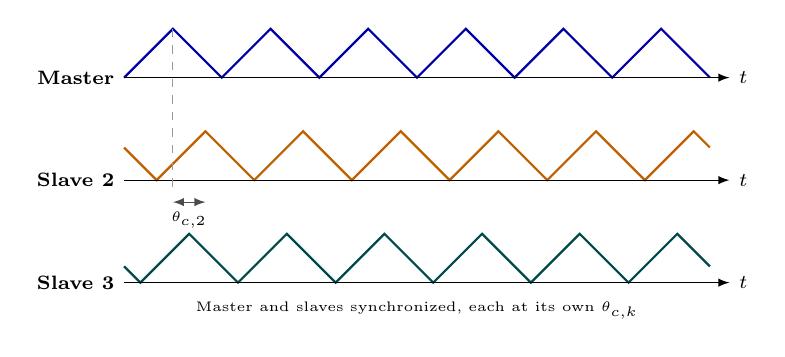
\begin{tikzpicture}[font=\scriptsize,x=6.2mm,y=6.2mm,>=latex]
% ---- Master carrier (blue), baseline y=0 ----
\draw[blue!65!black,thick]
  (0,0)--(1,1)--(2,0)--(3,1)--(4,0)--(5,1)--(6,0)
  --(7,1)--(8,0)--(9,1)--(10,0)--(11,1)--(12,0);
\draw[->] (0,0) -- (12.4,0) node[right] {$t$};
\node[left] at (0,0) {\textbf{Master}};
% ---- Slave 2 (orange), phase offset theta_c,2, baseline y=-2.1 ----
\draw[orange!75!black,thick]
  (0,-2.1+0.667)--(0.667,-2.1)--(1.667,-2.1+1)--(2.667,-2.1)
  --(3.667,-2.1+1)--(4.667,-2.1)--(5.667,-2.1+1)--(6.667,-2.1)
  --(7.667,-2.1+1)--(8.667,-2.1)--(9.667,-2.1+1)--(10.667,-2.1)
  --(11.667,-2.1+1)--(12,-2.1+0.667);
\draw[->] (0,-2.1) -- (12.4,-2.1) node[right] {$t$};
\node[left] at (0,-2.1) {\textbf{Slave 2}};
% ---- Slave 3 (teal), phase offset theta_c,3, baseline y=-4.2 ----
\draw[teal!58!black,thick]
  (0,-4.2+0.333)--(0.333,-4.2)--(1.333,-4.2+1)--(2.333,-4.2)
  --(3.333,-4.2+1)--(4.333,-4.2)--(5.333,-4.2+1)--(6.333,-4.2)
  --(7.333,-4.2+1)--(8.333,-4.2)--(9.333,-4.2+1)--(10.333,-4.2)
  --(11.333,-4.2+1)--(12,-4.2+0.333);
\draw[->] (0,-4.2) -- (12.4,-4.2) node[right] {$t$};
\node[left] at (0,-4.2) {\textbf{Slave 3}};
\node[below,font=\tiny] at (6,-4.4)
  {Master and slaves synchronized, each at its own $\theta_{c,k}$};
% ---- theta_c,2 annotation between master and slave-2 peaks ----
\draw[dashed,black!40,thin] (1,1) -- (1,-2.4);
\draw[<->,black!70] (1,-2.55) -- (1.667,-2.55);
\node[below,font=\tiny] at (1.33,-2.55) {$\theta_{c,2}$};
\end{tikzpicture}
\caption{Master/slave carrier synchronization for a representative
$N=3$ example: each slave's carrier is offset from the master by its
own phase $\theta_{c,k}$ \eqref{eq:carrier_phase}.}
\label{fig:carrier_sync_mechanism}
\end{figure}


\subsection{DC-Link Ripple Reduction and Battery-Side Current}

DC-link current ripple accelerates battery aging and is itself a
design objective. Lower-voltage cell switches typically enable a
higher switching frequency for a given loss budget, reducing the
required per-cell capacitance and battery-side ripple relative to a
single high-voltage bridge; carrier-phase interleaving reduces this
ripple further still.

The cell's dc-side current follows from convolving each phase's
switching-function spectrum with its current spectrum and summing over
the three phases,
\begin{equation}
I_{\mathrm{conv},x,k}=\tfrac12\left(S_{x,k}\otimes I_{x,k}\right).
\label{eq:conv_current_spectrum}
\end{equation}

For a single cell, every carrier harmonic $m$ contributes sidebands at
$n=\pm6p-3$ ($m$ odd) or $n=\pm6p$ ($m$ even), for integer $p$. With
uniform interleaving $\theta_{c,k}=2\pi k/N$, summing the $N$ cells'
converter currents shows that only carrier harmonics that are
themselves multiples of $N$ survive ($m=pN$ for even $N$, $m=2pN$ for
odd $N$), each retaining the same sideband structure
\cite{Jin2014Control}.


Translating this converter-current spectrum into the dc-link current
actually shared by the series stack requires the SPB equivalent
circuit of Section~\ref{sec:dclink_balancing},
\begin{equation}
L\frac{di_{\mathrm{dc}}}{dt}=E-Ri_{\mathrm{dc}}-\sum_kv_{\mathrm{conv},k},
\qquad
C_k\frac{dv_{\mathrm{conv},k}}{dt}=i_{\mathrm{dc}}-i_{\mathrm{conv},k},
\label{eq:dclink_ode}
\end{equation}
giving a closed-form transfer function between the summed
converter-current spectrum and the resulting dc-bus current
\cite{Jin2014Control},
\begin{equation}
I_{\mathrm{dc}}(\omega)=\frac{\sum_{k=1}^{N}I_{\mathrm{conv},k}(\omega)}
{N-\omega^2LC+j\omega CR}.
\label{eq:battery_current_tf}
\end{equation}
Because the residual dc-link ripple is dominated by the lowest
surviving harmonic, $m=N$, evaluating
\eqref{eq:battery_current_tf} there gives an approximate ripple
estimate,
\begin{equation}
\Delta i_{\mathrm{dc}}\approx\frac{\left|\sum_{k=1}^{N}
I_{\mathrm{conv},k}(2\pi Nf_{sw})\right|}
{\left|N-(2\pi Nf_{sw})^2LC+j2\pi Nf_{sw}CR\right|}.
\label{eq:dclink_ripple_estimate}
\end{equation}

Because the surviving harmonic sits at $N$ times the per-cell
switching frequency, both the removal of the uncancelled low-order
sidebands and the higher-frequency $LC$ attenuation act in the same
direction. Fig.~\ref{fig:dclink_ripple_interleaving} illustrates this
by simulation for a representative $N=3$ case.

\begin{figure}[!t]
\centering
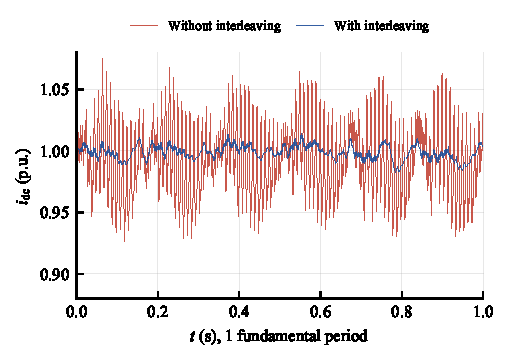
\includegraphics[width=\columnwidth]{Figures/fig_dclink_ripple.pdf}
\caption{Coupled circuit simulation of the shared series dc-link
current $i_{\mathrm{dc}}(t)$ for $N=3$ SPB cells ($M=0.85$,
$f_1=1$~Hz, $f_{sw}=100$~Hz), without (red) and with (blue) carrier
interleaving between submodules \eqref{eq:carrier_phase}. Both traces
share the same dc average; interleaving reduces the peak-to-peak
ripple by roughly $4$--$5\times$, consistent with
\eqref{eq:dclink_ripple_estimate}. Computed simulation result, not
measured hardware data.}
\label{fig:dclink_ripple_interleaving}
\end{figure}

This simulation lumps the battery-to-stack bus inductance but treats
each cell's own connection to that bus as ideal. In a physically
distributed implementation, each cell instead reaches the shared dc
path through its own bus-bar and connector loop, whose parasitic
inductance couples back into the cancellation mechanism itself: Wang
\textit{et al.} \cite{Wang2015GaNIMMD} found that a series-connected
GaN IMMD required careful capacitor selection and tight layout to
preserve the benefit of interleaving, and an earlier characterization
of an interleaved series-connected drive found that parasitic loop
inductance could make the interleaved ripple larger than the
non-interleaved case \cite{Wang2015ThesisDVB}. The reduction in
Fig.~\ref{fig:dclink_ripple_interleaving} should therefore be read as
an upper bound, with the achievable benefit set by layout, capacitor
selection, and switching frequency rather than by carrier phasing
alone.

\subsection{Machine Harmonics, Voltage Utilization, and Switching Loss}

The optimum carrier displacement is nonetheless
not universal: it depends on cell count, modulation index, power
factor, winding displacement, and the specific quantity being
minimized, so carrier coordination should be viewed as one design
variable within a larger converter--machine modulation problem.

SPB-specific studies show that inter-cell modulation affects both semiconductor losses and
dc-link-current harmonics \cite{Jin2017Modulation}, and related
modular and multiphase drives demonstrate simultaneous reduction of
dc-link and machine current ripple
\cite{Verkroost2021Ripple,DeMarcos2025InterleavedPWM,Wang2025HybridPWM}.

The multiphase machine makes the harmonic problem substantially more
involved than in a conventional three-phase drive: nonfundamental
voltage components can excite additional harmonic subspaces with low
impedance, producing copper loss and torque ripple even when
fundamental current control is fully satisfactory. Recent
integrated-modular-drive studies accordingly move toward interleaved
and discontinuous PWM techniques tailored to this multiphase
current-ripple problem
\cite{Hopkins2019DCLinkRipple,Mohamed2020DCLinkSizing,Alosa2019ModularRipple}.

At high speed, modulation must also maximize voltage utilization,
because each winding group is supplied only from its local cell
voltage $V_{\mathrm{dc},k}$, as constrained by
\eqref{eq:spb_machine_voltage_limit} -- an objective that grows more
important as $N$ increases and $V_{\mathrm{dc},k}$ falls accordingly.
Optimized vector selection for dual-three-phase traction machines has
demonstrated the possibility of extending the high-modulation region
while simultaneously suppressing unwanted subspace currents
\cite{Chen2026HighModulationDTP}.

Switching loss introduces an opposing objective. DPWM and hybrid
strategies reduce the number of transitions by clamping selected
phases or by redistributing high-frequency switching among converter
modules. Related open-end-winding (OEW) work demonstrates that
coordinated modulation can reduce switching loss and unwanted
zero-sequence current simultaneously \cite{Yang2026HybridOEW,
Lee2026AlternatingDPWM}; although its dc architecture differs, the
underlying principle of distributing switching activity among several
inverter modules is directly transferable to SPB.

\subsection{Coupling to Balancing and Common-Mode Objectives}

Modulation also sets the achievable authority for two further
objectives that are developed as dedicated topics later in this paper:
dc-link voltage balancing (Section~\ref{sec:dclink_balancing}), where
differential winding-group power must be realizable through modulation
without violating local voltage and current limits
\cite{Verkroost2024PowerDistribution,Wu2020ActiveBalancing,
Mocevic2024GateDelay}; and common-mode voltage (Section~\ref{sec:common_mode}),
where redundant voltage vectors or coordinated zero-sequence terms can
reduce frame excitation \cite{Sun2025CMVMPC,Zheng2025MultiObjectivePWM,
Chen2020EMCIntegrated}. 
The key SPB modulation question is therefore
not which conventional PWM method performs best in isolation, but how
switching decisions should be coordinated across cells to jointly
manage ripple, loss, balancing, and common-mode objectives over the
full operating map.
